\section{Deployment on FABRIC} \label{sec:fabric}
This section describes how we deployed Hydra the NSF FABRIC testbed\cite{8972790}.

\subsection{Hydra Deployment Overview}
As it shown in Figure \ref{fig:nodes-on-fabric}, We provisioned nodes on the NSF FABRIC (\url{https://fabric-testbed.net}) testbed as Hydra’s initial “soft” deployment. One node is a client node and others are hydra nodes. We choose five nodes because four nodes is the minimum number of nodes to demonstrate the Hydra function and one node as a client node. 

Our base FABRIC resource "slice" has the following properties:
\begin{itemize}
    \item Layer 2 connectivity (i.e. MAC address) to communicate, completely connected network graph, manual setup / routing.
    \item Easily deployed and destroyed to enable full system rebuilds for reproducibility testing. 
    \item High network bandwidth (100Gbps) links between nationally dispersed sites.
    \item Scalable resource allocation and modern hardware (e.g. NVME, GPUs, etc.) for the creation of a data lake of sufficient scale for data-intensive scientific workflows.
\end{itemize}

\begin{figure}[!ht]
    \centering
    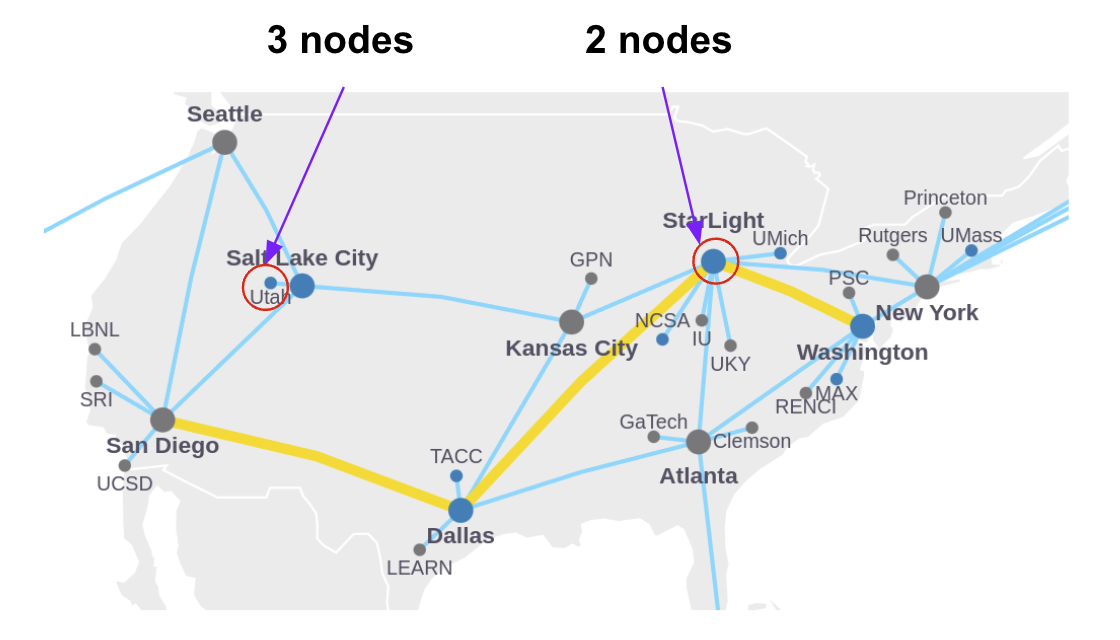
\includegraphics[width=\columnwidth]{visuals/deploy-on-fabric.png}
    \caption{Hydra deployment on the FABRIC testbed.}
    \label{fig:nodes-on-fabric}
\end{figure}

\lstset{
  aboveskip=1ex,
  %backgroundcolor=\color{gray!25},
  basicstyle=\small\ttfamily,
  belowskip=1ex,
  breaklines=true,
  columns=fullflexible,
  framerule=0pt,
  framexrightmargin=0em,
  framexleftmargin=0em,
  language=[LaTeX]TeX,
  %numbers=left,
  %numberstyle=\footnotesize\sffamily,
  tabsize=2
}

\subsection{Hydra Deployment on the FABRIC Testbed}
To deploy the program on Fabric, first we have to become Fabric users by simply signing up at \url{http://portal.fabric-testbed.net}. The second step is to join a project. Users can join an existing project or they can create a new one. Fabric has its own JupterHub, which makes users easily integrate with the Fabric environment. The next step is setting up two SSH keypairs: bastion keypaire and sliver keypaire. The bastion keypair can be generated from the Fabric portal but has a finite lifetime. Users need to re-generate their bastion keypairs every 3 months. The sliver keypairs are long lived and installed into VMs. The environment configuration is completed when users add the path of these two keypairs into the Juyperhub. In our experiment, we used the FABRIC API (https://github.com/fabric-testbed/fabrictestbed-extensions) to request a slice with five nodes with three nodes in Utah and two nodes in Illinois. The five nodes were set up with default components: two CPU cores, 8Gb RAM, and 10Gb SSD disk space.  A layer 2 network was built between these five nodes as shown in Figure \ref{fig:nodes-interface}. 

After the deployment of the slice with basic VMs, we installed the Hydra packages on each node as python3-pip, libndn-cxx-dev, nfd, ndnping, ndnpeek, ndn-dissect, ndnchunks and ndnsec. Then, we established Hydra python libraries by running a command:

\begin{lstlisting}[language=bash]
    node:$ pip3 install python-ndn ndn-storage ndn-svs ndn-hydra
\end{lstlisting}

Next we added the NDN face and route between the client node and the Hydra nodes as in Figure \ref{fig:nodes-interface}. The following command shows how to create face and add route between two hydra nodes (node 2 and node 3) :
\begin{lstlisting}[language=bash]
  node2:$ nfd-start
  node2:$ nfdc face create remote ether://["MAC address of node 3"] local dev://"Ethernet interface of node 2 with node 3"
  node2:$ nfdc route add /hydra/group ether://["MAC address of node 3"]
  node2:$ nfdc route add /hydra/node/node3 ether://["MAC address of node 3"]
  node2:$ nfdc route add /node3 ether://["MAC address of node 3"]
\end{lstlisting}

\noindent The following command shows how to create face and add route between a hydra node and a client node (node 2 and node 1) :
\begin{lstlisting}[language=bash]
  node2:$ nfd-start
  node2:$ nfdc face create remote ether://["MAC address of node 1"] local dev://"Ethernet interface of node 2 with node 1"
  node2:$ nfdc route add /client ether://["MAC address of node 1"]
\end{lstlisting}

Finally we moved data into and out of the Hydra deployment using 1MB, 5MB and 10 MB files for testing purposes.

\begin{figure}[!ht]
    \centering
    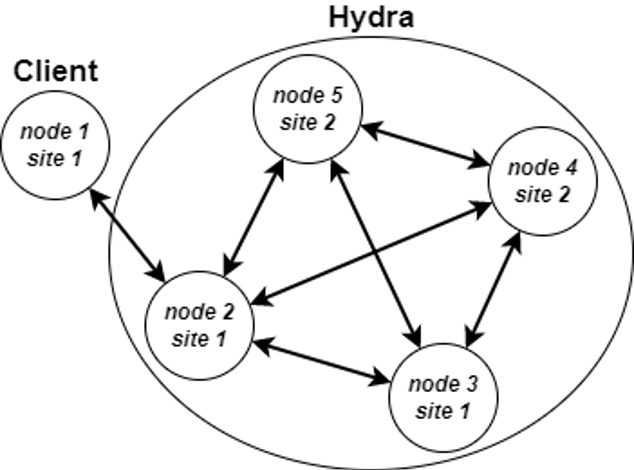
\includegraphics[width=0.8\columnwidth]{visuals/nodes-on-fabric.png}
    \caption{FABRIC topology overview of the client and Hydra nodes. }
    \label{fig:nodes-interface}
\end{figure}

\subsection{Proof of Principle Hydra Experiment }
In our proof of principle experiment, we achieved four functionalities: \textit{query}, \textit{insert}, \textit{fetch}, and \textit{delete}. Once all the Hydra nodes came online, we were able to validate internode communication and performance with \textit{iperf}. 

First, the client node sent the \textit{query} to the Hydra node by command:
\begin{lstlisting}[language=bash]
  node1:$ ndn-hydra-client query -r REPONAME -q QUERY [-n NODENAME]
\end{lstlisting}

This command helps the client check whether the required files are stored on Hydra nodes. 

The second test command is the \textit{insert} command: 
\begin{lstlisting}[language=bash]
  node1:$ ndn-hydra-client insert -r REPONAME -f FILENAME -p PATH
\end{lstlisting}
The client node could then publish data to Hydra nodes. Note that the data file was separated into several small chunks based on the file sizes and stored on Hydra nodes.

Next, we \textit{fetch} the file from the Hydra node by using the command: 
\begin{lstlisting}[language=bash]
  node1:$ ndn-hydra-client fetch -r REPONAME -f FILENAME [-p PATH]
\end{lstlisting}
Through this command, Hydra will link the client node with the node with the request file and the request file will be forwarded to the client node. 

After testing these three commands, the \textit{delete} command was used to remove all files on hydra nodes by using this command: 
\begin{lstlisting}[language=bash]
  node1:$ ndn-hydra-client delete -r REPONAME -f FILENAME
\end{lstlisting}


This basic procedure is being used to validate Hydra releases as well as vary testbed topology, slice hardware, dataset size, and data name schemas.